%中間審査概要テンプレート ver. 3.0

\documentclass[uplatex,twocolumn,dvipdfmx]{jsarticle}
\usepackage[top=22mm,bottom=22mm,left=22mm,right=22mm]{geometry}
\setlength{\columnsep}{10mm}
\usepackage[T1]{fontenc}
\usepackage{txfonts}
\usepackage[expert,deluxe]{otf}
\usepackage[dvipdfmx,hiresbb]{graphicx}
\usepackage[dvipdfmx]{hyperref}
\usepackage{pxjahyper}
\usepackage{secdot}


%タイトルと学生番号,名前だけ編集すること
\title{\vspace{-5mm}\fontsize{14pt}{0pt}\selectfont Wikipediaにおけるプロジェクトマネジメント状況の分析}
\author{\normalsize プロジェクトマネジメントコース 矢吹研究室 1342100 春川直幸}
\date{}
\pagestyle{empty}
\begin{document}
\fontsize{10.5pt}{\baselineskip}\selectfont
\maketitle


%以下が本文
\section{背景}

Wikipedia は,多くのボランティアにより,始まってから10 年足らずの間に,大きな成長を見せたオンライン百科事典プロジェクトである.総記事数の文字数は10 億文字を超え,ブリタニカ国際大百科事典とエンカルタ総合大百科の合計と比較しても上回る.Wikipedia は,さまざまな言語が参加しているグローバルなプロジェクトでもある\cite{wikirevo}.2016年2月現在では,291個もの言語で執筆が行われている.

既存の百科事典や他の類似のプロジェクトと比較した場合,Wikipediaには次のような特徴がある.
従来,専門家によって監修,編集される百科事典を一般のインターネット利用者が匿名で編集できるようにしていること.参加者の資格制限などを行っていないため,年齢,職業,国籍などの点で多様な執筆者がボランティアで編集に関わることができるといった特徴がある\cite{wiki}.

記事の内容はボランティアの人々の協力により加筆や修正,削除が行われている.
誰でも自由に編集できるからこそ,記事編集の貢献度が曖昧になってしまっている.

本研究では,Wikipediaの編集履歴データをマイニングすることによって,Wikipediaにおけるプロジェクトマネジメントの状況を分析する.




\section{目的}

Wikipediaを一つのプロジェクトとみなし,このオンライン百科事典でのプロジェクトマネジメント状況を調査する.この調査によりオープンな共同プロジェクトにおける,プロジェクトマネジメントの状況についての知見を得たい.

\section{手法}

\begin{enumerate}
 \item Wikipedia日本語版の編集履歴を取得し,データマイニングを行う.
 \item オープンなプロジェクトにおけるプロジェクトマネジメントの状況を分析する.
\end{enumerate}

\section{想定される成果物}

編集履歴に関するデータを収集し,編集回数や版の情報量などの要素を洗い出す.そして,ヒストグラムを作成する.その結果から,
Wikipediaのオープンなプロジェクトでのプロジェクトマネジメント状況の知見を得る.

\begin{figure}[h]
\centering
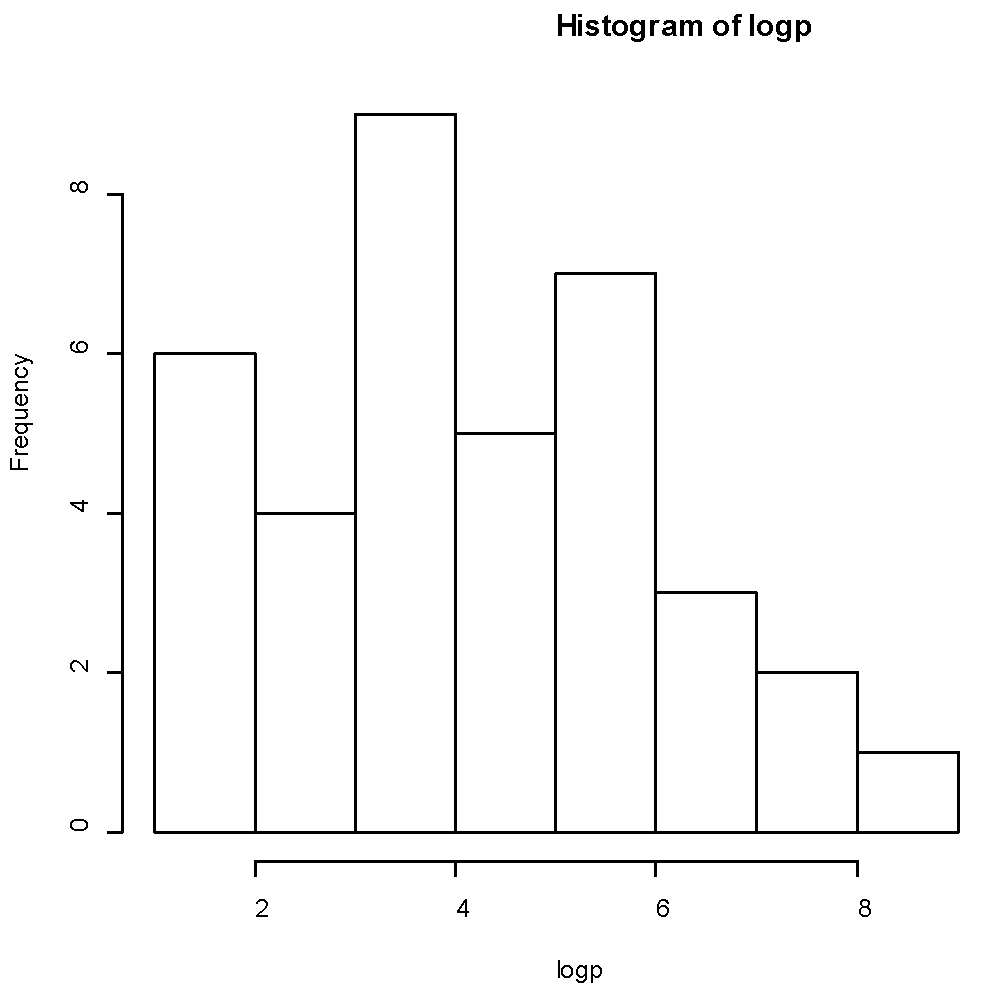
\includegraphics[width=6cm,clip]{figure1.pdf}
\caption{ヒストグラム}\label{サンプル図}
\end{figure}

\section{進捗状況}

編集履歴を取得し分析するため,Rを使用しヒストグラムを作成した.


\section{今後の計画}

以下の順番で行う.

\begin{enumerate}

 \item Wikipediaの編集履歴データを取得する.
 \item Wikipediaの編集履歴データを解析し,オープンなプロジェクトをする際のプロジェクトマネジメントの状況を調査,分析する.

\end{enumerate}


\bibliographystyle{junsrt}
\bibliography{biblio}%「biblio.bib」というファイルが必要.

\end{document}
